\documentclass{beamer}

\usetheme{Antibes}
%\usetheme{split}
% this is a template for slides using beamer package
% adapted from slides written by Ramon Medrado
% first version: Ana Bazzan
\usecolortheme[RGB={120,0,0}]{structure}
\setbeamertemplate{blocks}[rounded][shadow=true]
\usepackage[latin1]{inputenc}
\usepackage{ragged2e}
\usepackage{graphicx}
\usepackage{caption}
\usepackage{booktabs}
\usepackage{subfig}
\usepackage{cite}

\begin{document}
\title{Work in progress}

\section{Pipeline steps}
\frame{\frametitle{Pipeline steps}
	\begin{columns}
		\begin{column}{0.5\textwidth}
			\begin{itemize}
				\justifying
				\item Estimating surface normals using PCA of covariance matrix;
				\item Testing a local 3D descriptor, CoSPAIR (2016):
				\begin{itemize}
					\justifying
					\item ISS3D keypoint detection;
					\item Support radius divided into N concentric spheres;					
					\item Histograms of spatial concentric oriented surface points (surflet) pairs relation at each sphere;
					\item Color histograms for each channel at each sphere;		
				\end{itemize}								
			\end{itemize}
		\end{column}
		\begin{column}{0.5\textwidth}  %%<--- here
			\begin{center}
				\begin{figure}[ht]
					\centering
					\label{figure:fig1}
					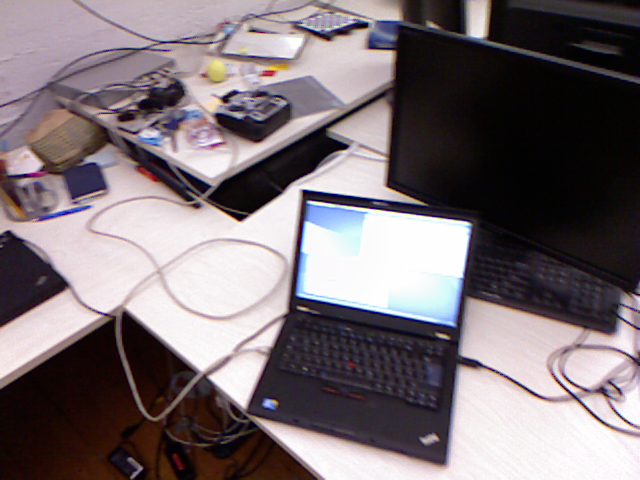
\includegraphics[scale=0.35, height=60pt, width=80pt]{rgb}
					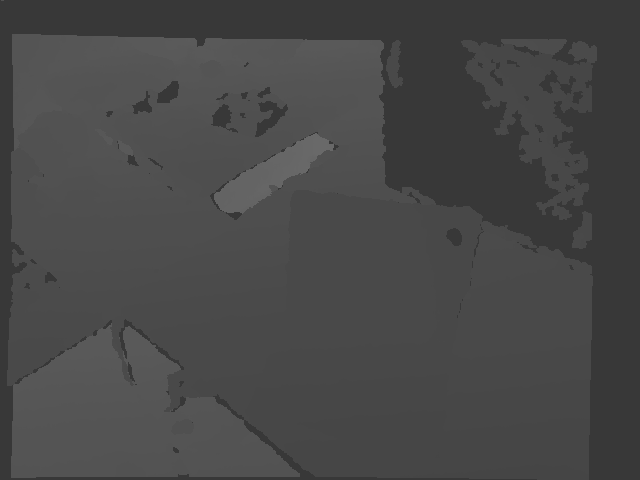
\includegraphics[scale=0.35, height=60pt, width=80pt]{depth}
					
					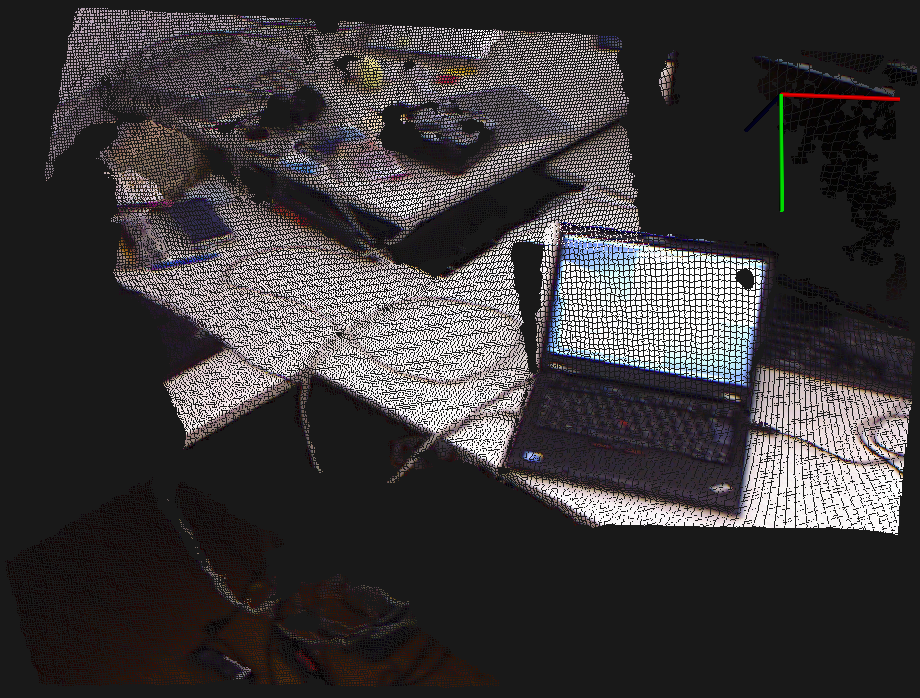
\includegraphics[scale=0.35, height=80pt, width=120pt]{cloud}
					\small
					\caption{RGB, depth and point cloud.}	
				\end{figure}
			\end{center}
		\end{column}
	\end{columns}
}

\section{Pipeline steps}
\frame{\frametitle{Pipeline steps}
	\begin{columns}
		\begin{column}{\textwidth}
			\begin{itemize}
				\justifying
				\item Matching with L2-norm, querying using linear search or FLANN kdtree with k-nearest neighbors;
				\item Rejecting matched outliers with Lowe (1999) distance ratio check;
				\item Selecting best candidate with a naive voting scheme, aggregating votes using each inlier's match only.
			\end{itemize}
		\end{column}
	\end{columns}
}

\section{Next steps}
\frame{\frametitle{Next steps}
	\begin{columns}
		\begin{column}{\textwidth}
			\begin{itemize}
				\justifying
				\item Normal estimation (ex.: using integral images for organized point clouds (2013));
				\item Keypoint detection (ex.: alternative method or detection strategy);
				\item Local or global descriptors (or "turning" local into a global one by manipulating support sizes);
				\begin{itemize}
					\justifying
					\item Shape and color preferred, making use of the RGB-D input;
				\end{itemize}
							
				\item Querying strategy (ex.: alternative tree structures, inverted multi-index);
				\item Rejecting outliers (ex.: alternative checks, SAC variants);
				\item Voting scheme (ex.: probabilistic voting (2017)). 
			\end{itemize}
		\end{column}
	\end{columns}
}

\nocite{*}

\end{document}




